% Early Science Data Products
% Responsible: Leanne Guy
\section{Early Science Data Products}
\label{sec:data}

Here we provide a summary of the data products that are expected to be made available as part of the \esp.
The definitive source for all LSST data products is the Data Products Definition Document, \citep{LSE-163}.
The Rubin data rights policy is described in  \cite{RDO-013}.

\subsection{Prompt data products}

Prompt data products are described in detail in the Data Products Definition Document (\DPDD).
Alert packets are triggered by difference image source detections and transmitted to community alert brokers\footnote{See \url{https://www.lsst.org/scientists/alert-brokers} for the list of selected brokers.} and are publicly available.
Similarly, daily Solar System Processing identifies new Solar System Objects from difference image sources and reports those publicly to the Minor Planet Center.

Catalog and image products, as well as services for running user-generated processing on the data, are available to Rubin Data Rights holders after 24 hours through the Rubin Science Platform (\S~\ref{ssec:dataaccess}).
\DIASource, \DIAObject, and \SSObject catalogs are queryable using VO interfaces to the Prompt Products Database.

\subsection{Data Release data products}
Static science datasets for Early Science will flow from the \svs in commissioning.
Images and catalogs from the DRP of the commissioning data will be made available to data rights holders in the form of Data Previews via the access mechanisms described in \ref{ssec:dataaccess}.
Due to the relatively short time periods available for commissioning observations (\S \ref{ssec:scenarios}), these Data Previews will necessarily be limited in their area and temporal coverage relative to full Data Releases, however all Data Preview data products will be in the same science data model format as for future Data Releases.

\subsection{Access to \es data products}\label{ssec:dataaccess}
Alerts will be accessible by the community via one or more of the nine Rubin-endorsed Community Brokers.
The Rubin Data Rights community will access the Rubin data products via the Rubin Science Platform, \citep{LSE-319}.

\subsection{Summary of expected \es data products}

The tables in this section outline which data products can be expected in each \es data preview and data release, and when.

\begin{table}
\caption{Summary of data products expected in each data preview and early survey data release, as of October 2022.}
\label{tab:summary}
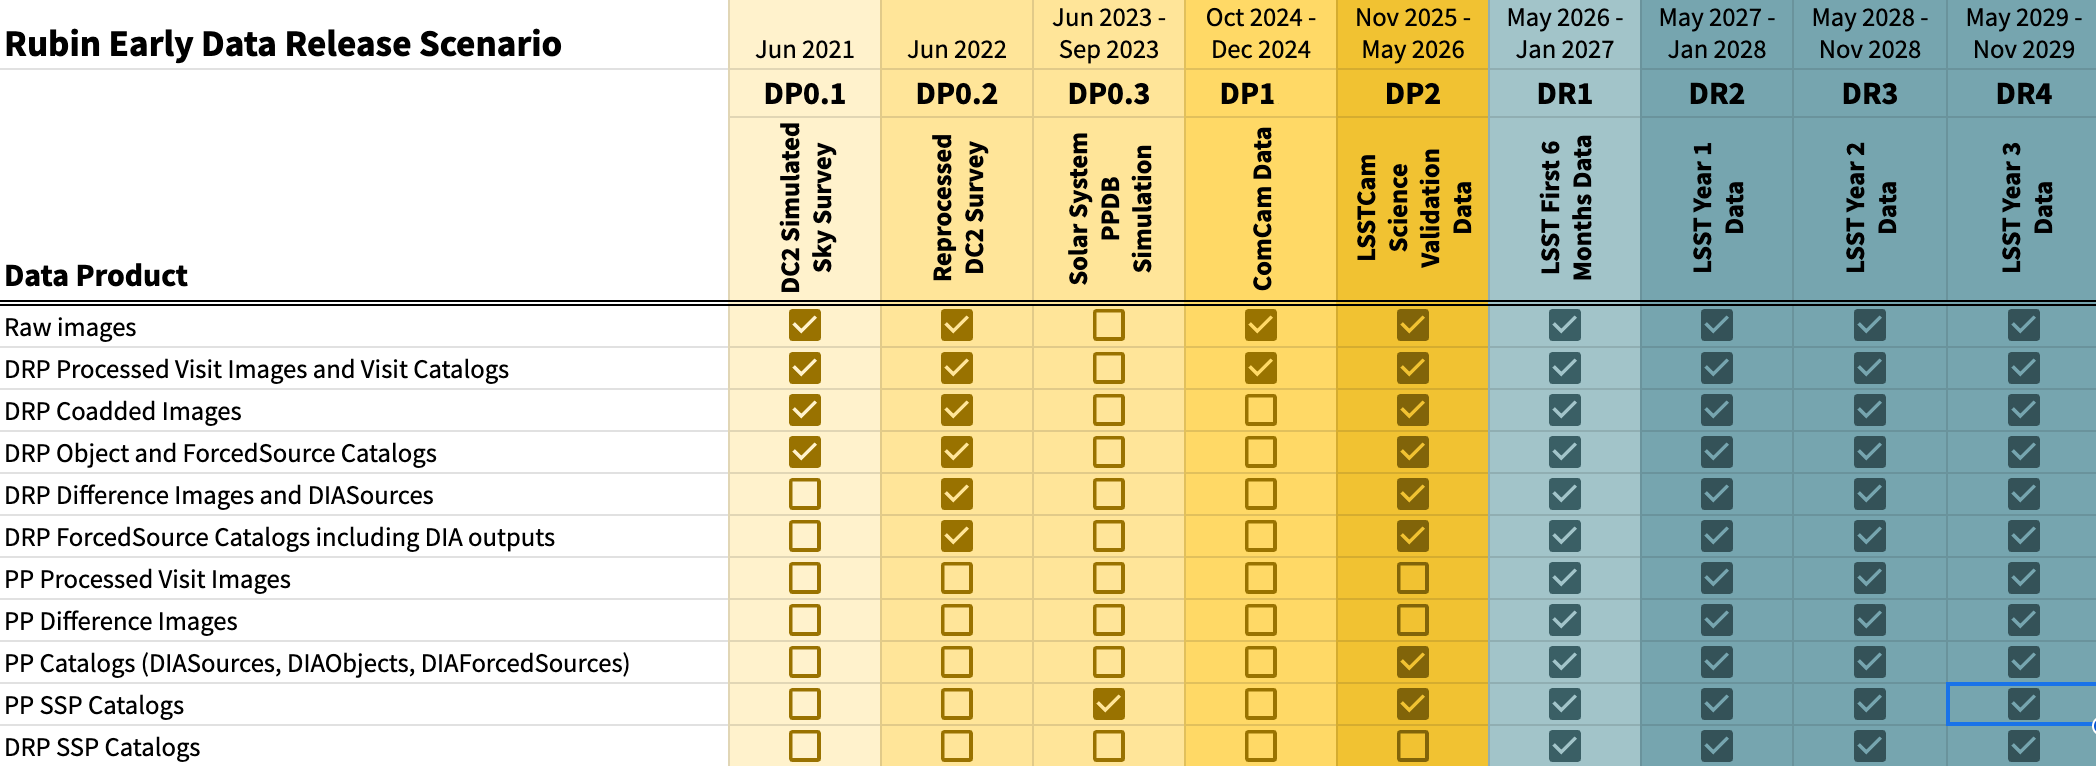
\includegraphics[width=\linewidth]{figures/DPR-summary}
\end{table}

\begin{table}
\caption{Summary of data products expected in DP1, as of October 2022.}
\label{tab:dp-one-products}
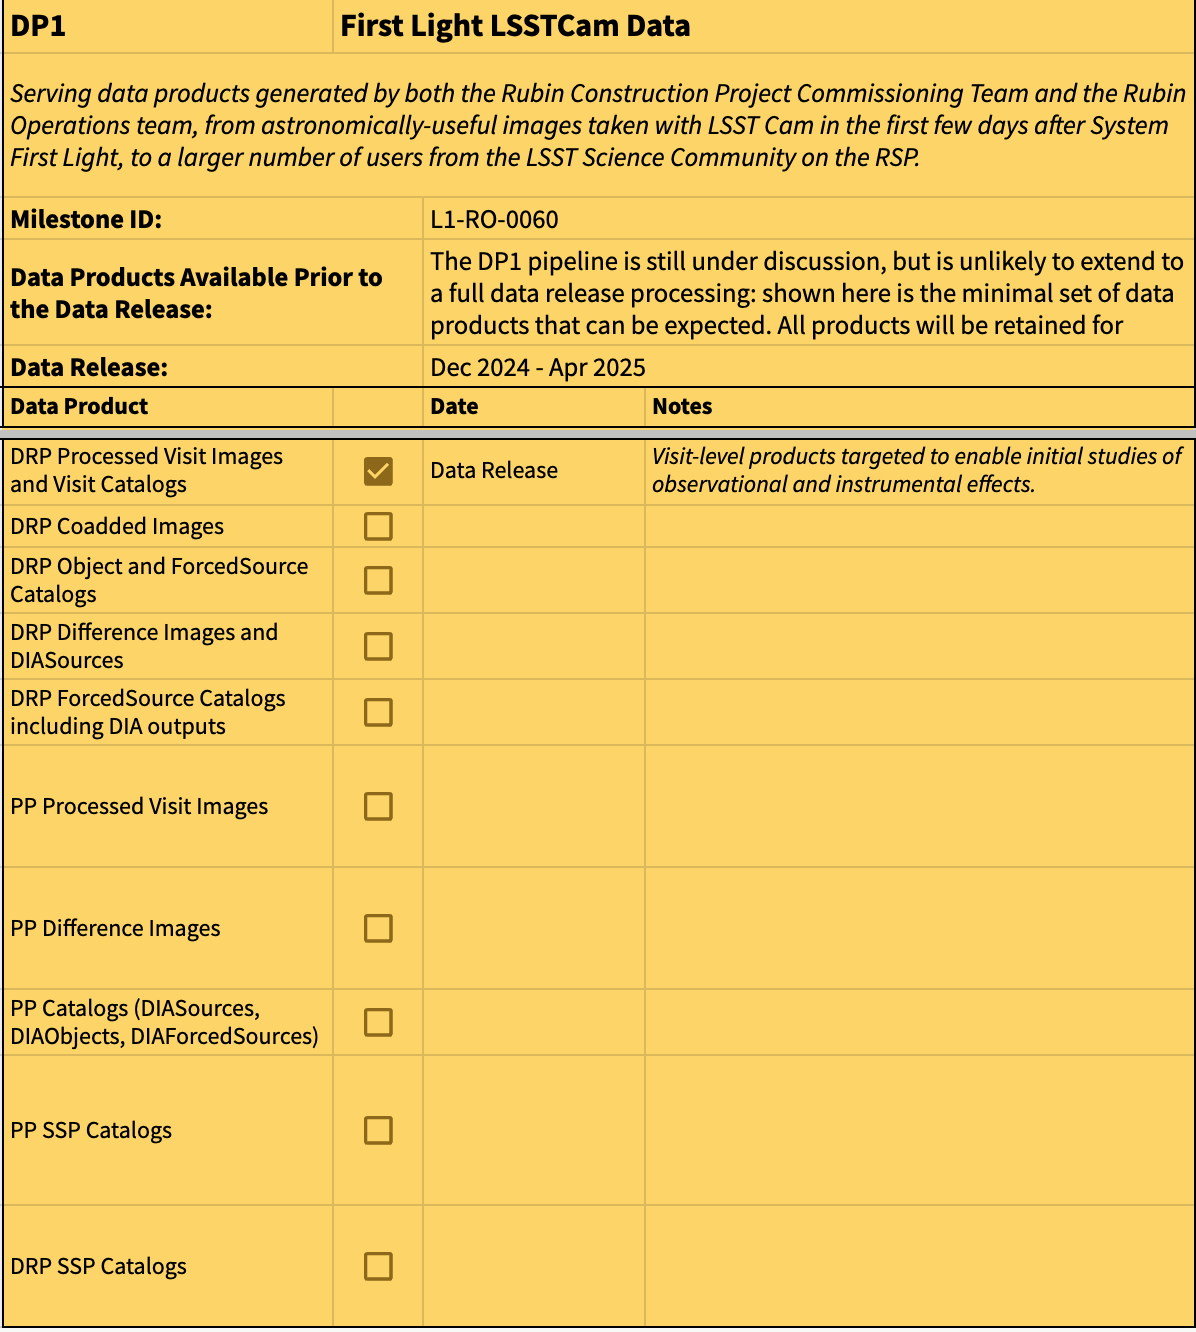
\includegraphics[width=\linewidth]{figures/DP1-products}
\end{table}

\begin{table}
\caption{Summary of data products expected in DP2, as of October 2022.}
\label{tab:dp-two-products}
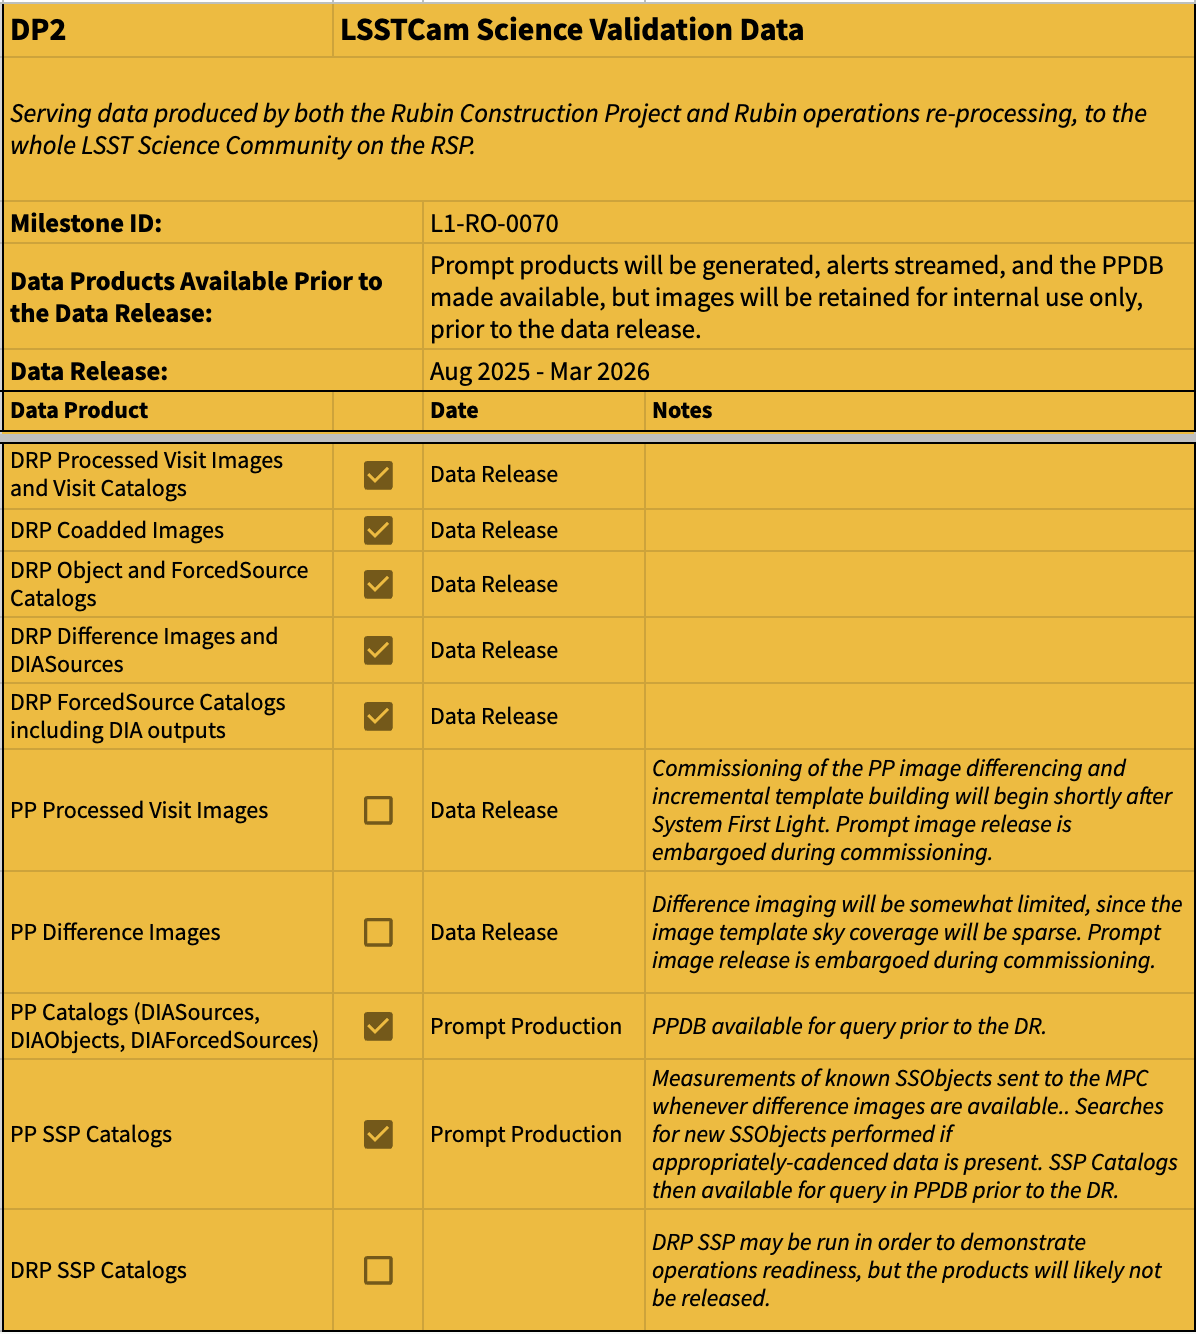
\includegraphics[width=\linewidth]{figures/DP2-products}
\end{table}

\begin{table}
\caption{Summary of data products expected in DR1, as of October 2022.}
\label{tab:dr-one-products}
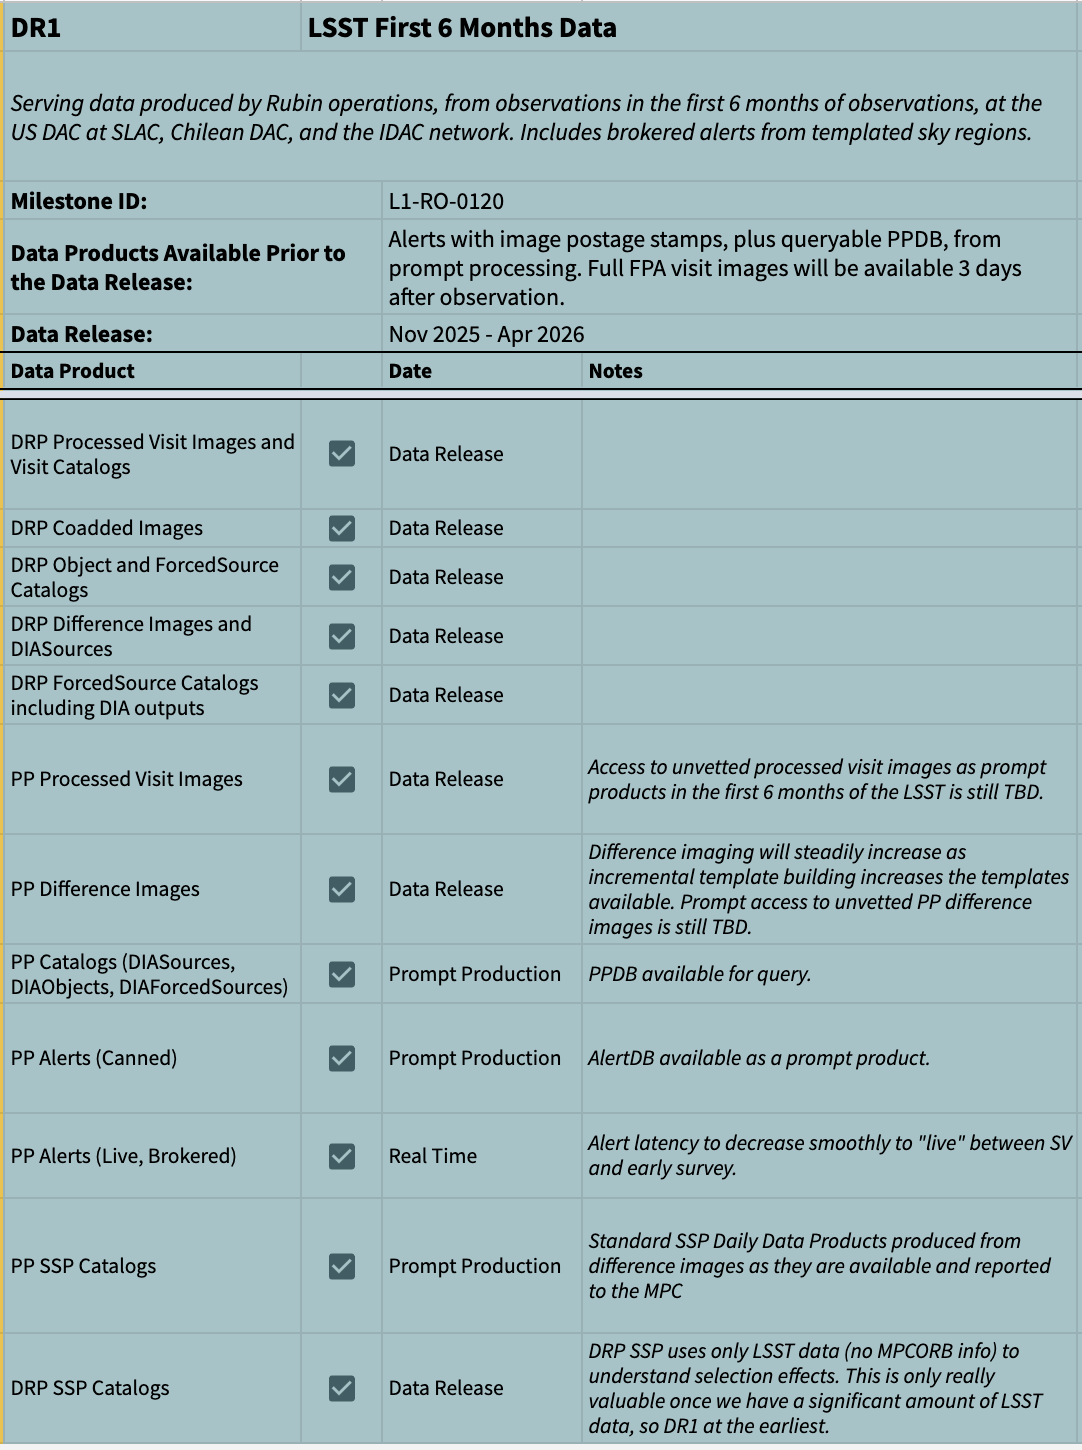
\includegraphics[width=\linewidth]{figures/DR1-products}
\end{table}
